\documentclass[8pt,a4paper,compress]{beamer}

\usepackage{/home/siyer/lib/slides}

\title{Hash Tables}
\date{}

\begin{document}
\begin{frame}
\vfill
\titlepage
\end{frame}

\begin{frame}
\frametitle{Outline}
\tableofcontents
\end{frame}

\section{Hashing}
\begin{frame}[fragile]
\pause

The basic idea is to save items in a key-indexed array, where the index is a function of the key

\pause
\bigskip

Hash function provides a method for computing an array index from a key

\pause
\bigskip

Issues
\begin{itemize}
\item Computing the hash function

\item Equality test: method for checking whether two keys are equal

\item Collision resolution: algorithm and data structure to handle two keys that hash to the same array index
\end{itemize}

\pause
\bigskip

Classic space-time tradeoff
\begin{itemize}
\item No space limitation: trivial hash function with key as index

\item No time limitation: trivial collision resolution with sequential search

\item Space and time limitations: hashing (the real world)
\end{itemize}
\end{frame}

\begin{frame}[fragile]
\pause

Idealistic goal: scramble the keys uniformly to produce a table index that is
\begin{itemize}
\item Efficiently computable

\item Equally likely for each key
\end{itemize}

\pause
\bigskip

Example 1: phone numbers
\begin{itemize}
\item Bad: first three digits

\item Better: last three digits
\end{itemize}

\pause
\bigskip

Example 2: social security numbers
\begin{itemize}
\item Bad: first three digits

\item Better: last four digits
\end{itemize}

\pause
\bigskip

Practical challenge: need different approach for each type of key
\end{frame}

\begin{frame}[fragile]
\pause

Java's hash code conventions
\begin{itemize}
\item All Java classes inherit a method \lstinline{hashCode()}, which returns a 32-bit \lstinline{int}

\item Requirement: if \lstinline{x.equals(y)}, then \lstinline{x.hashCode() == y.hashCode()}

\item Highly desirable: if \lstinline{!x.equals(y)}, then \lstinline{x.hashCode() != y.hashCode()}

\item Default implementation: return memory address of \lstinline{x}

\item Legal (but poor) implementation: always return 17

\item Customized implementations: \lstinline{Integer}, \lstinline{Double}, \lstinline{String}, \lstinline{File}, \lstinline{URL}, \lstinline{Date}, ...

\item User-defined types: users are on their own
\end{itemize}
\end{frame}

\begin{frame}[fragile]
\pause

Java library implementations
\begin{lstlisting}[language=Java]
public final class Boolean {
    private final boolean value;

    public int hashCode() { return value ? 1231 : 1237; }
}
\end{lstlisting}

\pause

\begin{lstlisting}[language=Java]
public final class Integer {
    private final int value;

    public int hashCode() { return value; }
}
\end{lstlisting}

\pause

\begin{lstlisting}[language=Java]
public final class Double {
    private final double value;

    public int hashCode() {
        long bits = doubleToLongBits(value);
        return (int) (bits ^ (bits >>> 32));
    }
}
\end{lstlisting}

\pause

\begin{lstlisting}[language=Java]
public final class String {
    private int hash = 0;
    private final char[] s;

    public int hashCode() {
        if (hash != 0) { return hash; }
        for (int i = 0; i < length(); i++) { hash = s[i] + (31 * hash); }
        return hash;
    }
} 
\end{lstlisting}
\end{frame}

\begin{frame}[fragile]
\pause

Implementing hash code for user-defined types
\begin{lstlisting}[language=Java]
public final class Transaction implements Comparable<Transaction> {
    private final String who;
    private final Date when;
    private final double amount;

    public int hashCode() {
        int hash = 17;
        hash = 31 * hash + who.hashCode();
        hash = 31 * hash + when.hashCode();
        hash = 31 * hash + ((Double) amount).hashCode();
        return hash;
    }
}
\end{lstlisting}

\pause
\bigskip

Hash code design
\begin{itemize}
\item Combine each significant field using the $31x + y$ rule

\item If field is a primitive type, use wrapper type \lstinline{hashCode()}

\item If field is \lstinline{null}, return 0

\item If field is a reference type, use \lstinline{hashCode()}

\item If field is an array, apply to each entry
\end{itemize}
\end{frame}

\begin{frame}[fragile]
\pause

Modular hashing
\begin{itemize}
\item Hash code: an \lstinline{int} between $-2^{31}$ and $2^{31} - 1$

\item Hash function: an \lstinline{int} between 0 and $M-1$ (for use as array index)
\end{itemize}

\pause
\bigskip

Implementation

\begin{lstlisting}[language=Java]
private int hash(Key key) { 
    return (key.hashCode() & 0x7fffffff) % M;
}
\end{lstlisting}

\pause
\bigskip

Uniform hashing assumption: each key is equally likely to hash to an integer between 0 and $M-1$

\pause
\bigskip

Example (hash value frequencies for words in Tale of Two Cities; 10,679 keys; $M = 97$)

\begin{center}
\visible<5->{\includegraphics[scale=0.35]{./figures/uniform_hashing.png}}
\end{center}

\pause
\bigskip

Collision: two distinct keys hash to the same index
\begin{itemize}
\item Can't avoid collisions unless you have a ridiculous amount of memory

\item Collisions are evenly distributed

\item Challenge: deal with collisions efficiently
\end{itemize}
\end{frame}

\section{Separate-Chaining Symbol Table}
\begin{frame}[fragile]
\pause

Use an array of $M < N$ linked lists
\begin{itemize}
\item Hash: map key to integer $i \in [0, M - 1]$

\item Insert: put at front of $i$th chain (if not already there)

\item Search: need to search only the $i$th chain
\end{itemize}

\begin{center}
\visible<2->{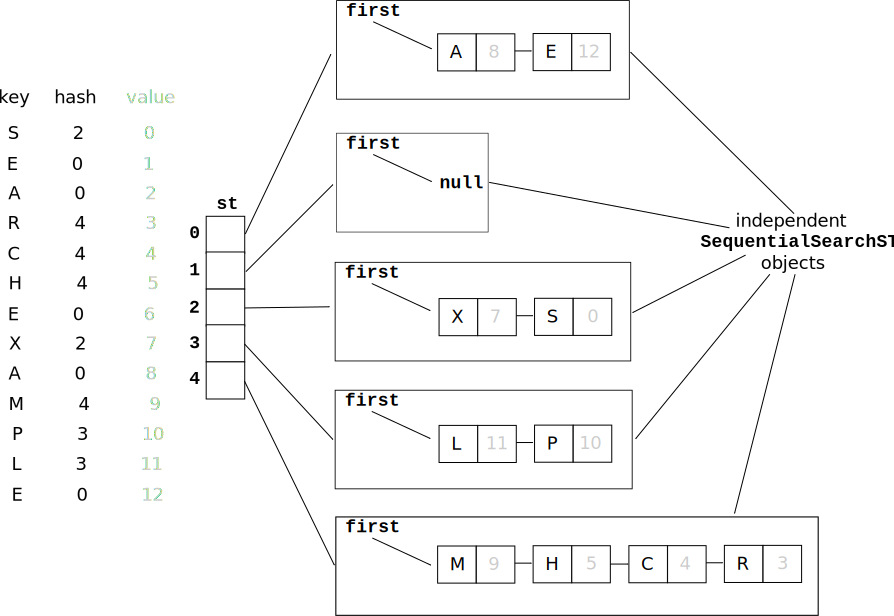
\includegraphics[scale=0.3]{./figures/separate_chaining.pdf}}
\end{center}

\pause
\bigskip

The ratio $N / M$ is called the load factor and is denoted by $\alpha$, and is interpreted as the average number of keys per list
\end{frame}

\begin{frame}[fragile]
\pause

Under uniform hashing assumption, probability that the number of
keys in a list is within a constant factor of $\alpha$ is extremely close to 1

\pause
\bigskip

Consequence: number of probes for search/insert is proportional to $\alpha$
\begin{itemize}
\item $M$ too large $\implies$ too many empty chains

\item $M$ too small $\implies$ chains too long
\end{itemize}

\pause
\bigskip

Goal: $\alpha = $ constant
\begin{itemize}
\item Double the size of array when $\alpha \geq 10$

\item Halve the size of array when $\alpha \leq 2$

\item Need to rehash all keys when resizing
\end{itemize}

\pause
\bigskip

Deleting a key (and its associated value) is easy --- need only consider chain containing key

\pause
\bigskip

The cost of search, insert, and delete, under the uniform hashing assumption, is constant (between 3 and 5)
\end{frame}

\begin{frame}[fragile]
\pause

\begin{lstlisting}[language=Java]
package edu.princeton.cs.algs4;

public class SeparateChainingHashST<Key, Value>  {
    private static final int INIT_CAPACITY = 4;
    private int N;
    private int M; 
    private SequentialSearchST<Key, Value>[] st; 

    public SeparateChainingHashST() { this(INIT_CAPACITY); } 

    public SeparateChainingHashST(int M) {
        this.M = M;
        st = (SequentialSearchST<Key, Value>[]) new SequentialSearchST[M];
        for (int i = 0; i < M; i++) { 
            st[i] = new SequentialSearchST<Key, Value>(); 
        }
    } 

    private void resize(int chains) {
        SeparateChainingHashST<Key, Value> temp = 
            new SeparateChainingHashST<Key, Value>(chains);
        for (int i = 0; i < M; i++) {
            for (Key key : st[i].keys()) { temp.put(key, st[i].get(key)); }
        }
        this.M  = temp.M;
        this.N  = temp.N;
        this.st = temp.st;
    }
    
    public int size() { return N; } 

    public boolean isEmpty() { return size() == 0; }
\end{lstlisting}
\end{frame}

\begin{frame}[fragile]
\pause

\begin{lstlisting}[language=Java]
    public boolean contains(Key key) { return get(key) != null; } 

    public Value get(Key key) {
        int i = hash(key);
        return st[i].get(key);
    } 

    public void put(Key key, Value val) {
        if (val == null) {
            delete(key);
            return;
        }
        if (N >= 10 * M) { resize(2 * M); }
        int i = hash(key);
        if (!st[i].contains(key)) { N++; }
        st[i].put(key, val);
    } 

    public void delete(Key key) {
        int i = hash(key);
        if (st[i].contains(key)) { N--; }
        st[i].delete(key);
        if (M > INIT_CAPACITY && N <= 2 * M) { resize(M / 2); }
    } 

    public Iterable<Key> keys() {
        Queue<Key> queue = new Queue<Key>();
        for (int i = 0; i < M; i++) {
            for (Key key : st[i].keys()) { queue.enqueue(key); }
        }
        return queue;
    } 
}
\end{lstlisting}
\end{frame}
\end{document}
